\chapter{Spatial clustering for docking solution ensemble interpretation}
\label{chapter:clustering}

In this chapter I describe why the conduction of a meaningful docking study
requires proper creation and analysis of an ensemble of docking solutions and
explain why clustering is an essential step for making reasonable predictions
about where and how a ligand binds to its receptor. This topic is unfortunately
not well discussed in current molecular docking literature, and existing
technical implementations for the clustering of docking solutions often do not
fit the scientific question and therefore may produce misleading results. Here,
I present a method optimized for clustering docking solution ensembles of GAG
molecules.

\section{Relevance of docking solution ensemble clustering}
\label{relevance_of_clustering}

In the framework of this thesis the term \enquote{docking solution} shall be
understood as a set of ligand atom coordinates, i.e.\ the spatial arrangement of
ligand atoms in the reference coordinate system as defined by the receptor
molecule. As a result of the statistical nature of the docking problem and the
use of pseudo random numbers in implementations of common docking search
algorithms, independent runs of the same docking method are expected to produce
different docking solutions. That is why for seeing the full picture, a
molecular docking method should be applied repetitively, resulting in an
ensemble of docking solutions.

The spatial distribution of docking solutions in that ensemble is governed by a
certain previously unknown probability distribution, which itself is implicitly
determined by the molecular interaction model and search algorithm implemented
in the docking method. Given that we trust the molecular interaction model, the
ultimate goal of a docking study is to obtain the global maximum (and/or some
local maxima) of the named probability distribution. Concept-wise, this is
equivalent to searching the state with highest probability, i.e. lowest energy.
Obtaining local maxima requires complete sampling of that unknown probability
distribution. That is why a docking method must be repeated until convergence
in the spatial distribution of the docking solutions is achieved. Only then the
ensemble reproduces the previously unknown probability distribution and reflects
the molecular interaction model as implemented by the docking method.

If convergence is observed, the next step is to identify the local maxima in the
spatial probability distribution of docking solutions. This problem can be
reformulated in terms of density, i.e.\ as finding the densest agglomerations of
docking solutions in the ensemble. However, a simple evaluation of the
distribution of atoms or molecules per volume would not provide useful results,
because a ligand molecule is comprised of multiple different atoms and has
various asymmetries with respect to shape and property. Spoken freely, the task
is to find agglomerations of docking solutions that are highly \textit{similar}
to each other. Hence, a promising approach is to evaluate the density in terms
of the \textit{similarity} between any two given docking solutions in the
ensemble, subject to the condition that a meaningful molecular similarity
measure can be found. In an abstract sense, the task is to identify groups of
highly similar docking solutions and to separate them from the bulk. This task
fits the general description of \textit{data clustering} as found in
\cite{tan_data_mining}:

\begin{adjustwidth}{1.5cm}{1.5cm}
\textit{%
\enquote{The goal is that the objects within a group be similar to one another
and different from the objects in other groups. The greater the similarity (or
homogeneity) within a group and the greater the difference between groups, the
better or more distinct the clustering.}}
\end{adjustwidth}

In conclusion, the most probable ligand molecule placement as predicted by a
certain docking method can be found by \textit{meaningful} clustering of the
converged ensemble of docking solutions. Meaningful clustering can be achieved
by selecting a problem-adjusted clustering method, whereas any data clustering
method has only two major components:

\begin{itemize}
\item the \textit{distance metric}, quantifying the similarity between any two
given objects.
\item a \textit{clustering algorithm}, classifying the objects into groups
(clusters), based on their mutual similarity.
\end{itemize}

It is important to appreciate that both components must be adjusted to the
scientific question, otherwise the result of docking solution clustering might
be meaningless. Within the next sections, I introduce a distance metric
optimized for GAG molecules and describe a clustering algorithm appropriate for
clustering molecular structure ensembles.


\section{A meaningful distance metric for GAGs: RMSatd}

As stated above, spatial clustering evaluates distances between data points
rather than data points themselves. No other information is available to the
clustering algorithm, so the distance metric alone must properly reflect the
similarity between two molecular structures, whereas a large similarity
obviously must correspond to a small distance.

The established way for measuring a structural distance between two molecules
that have an equivalent atomic configuration but different atomic coordinates is
to calculate the root mean square distance ($RMSd$) while pairing up atoms of
equivalent identity:

\begin{equation}
RMSd = \sqrt{\frac{1}{N}\sum{{d_i}^2}}
\end{equation}

Here, each of the $N$ atoms has its own identity and is unambiguously defined by
a unique identifier $i$. $d_i$ is the euclidean distance between two atoms of
the same identity, one in the first structure and the other in the second
structure. This classical $RMSd$ distance metric is for example used in
AutoDockTools \cite{autodock4_adt_2009} for docking solution clustering.

\begin{figure}
\centering
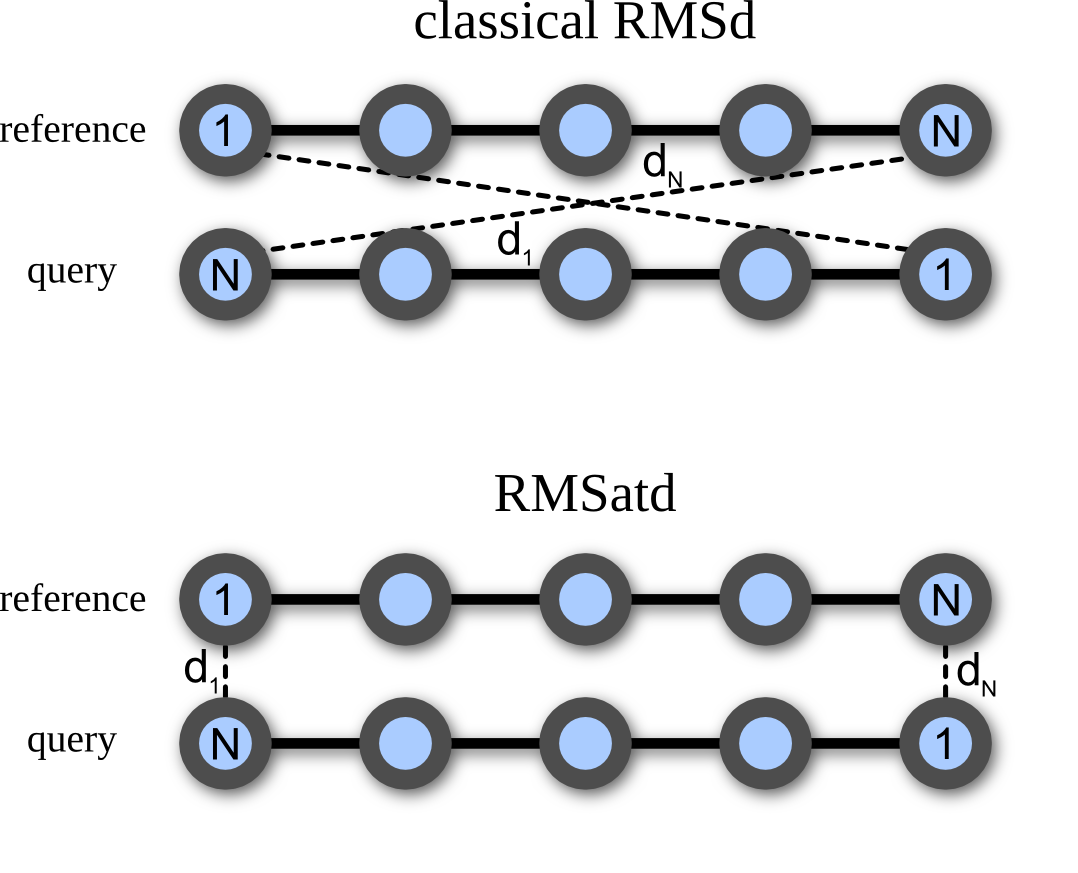
\includegraphics[width=0.7\textwidth]{gfx/clust/RMSd_vs_RMSatd_scheme_03.png}
\caption[]{
Schematic comparison of identity-based atom matching (classical $RMSd$)
\textit{vs.} type-based atom matching ($RMSatd$) by means of an extreme case,
where a linear molecule is compared to itself, after slight vertical shifting
and end-to-end inversion. All atoms (blue) are of the same type. Thick lines
indicate atomic bonds, $1 \dots N$ indicate atom identity. Dashed lines and
$d_i$ indicate pairwise distances used for building the $RMSd$ / $RMSatd$. Top
($RMSd$): atoms of same identity are paired up. Bottom ($RMSatd$): spatially
closest atoms of the same type are paired up.
}
\label{fig:clust:rmsd_vs_rmsatd}
\end{figure}

While the comparison by atom identity makes sense for large molecules such as
proteins, in more simple cases the classical $RMSd$ distance metric might not
properly reflect molecular similarity. This shall be demonstrated by means of an
extreme case, as indicated in the top panel of
\cref{fig:clust:rmsd_vs_rmsatd}. There, a molecule is comprised of linearly
chained atoms of the same type. That molecule exhibits a 2-fold rotational
symmetry: the atomic properties are invariant under the corresponding symmetry
operation (rotation by \SI{180}{\degree}, i.e.\ reversed directionality).
Although the two molecules are positioned almost equivalently, the classical
$RMSd$ measures quite a large distance, i.e.\ low similarity. Assuming bond
lengths and a vertical displacement between both molecules of \SI{1}{\angstrom},
the classical $RMSd$ in that situation would be \SI{3}{\angstrom}.

I propose what I call the \textit{root mean square atom type distance}
($RMSatd$), which works just as the classical $RMSd$, but pairs up spatially
closest atoms of the same type (\cref{fig:clust:rmsd_vs_rmsatd}, bottom panel).
In case of the example situation discussed above, the $RMSatd$ is
\SI{1}{\angstrom}, i.e.\ more realistically reflects the actual distance between
both molecules than the classical $RMSd$. While GAGs do not have a strict 2-fold
rotational symmetry, they are still highly similar when reversed along
their end-to-end direction. As demonstrated, this effect is accounted for by the
$RMSatd$ metric. Furthermore, GAGs are usually modeled as strictly periodic
molecules. The $RMSatd$ accounts for this periodicity and considers two GAGs
shifted by $n$ periodic units as structurally similar, while classical $RMSd$
with identity-based matching ignores this characteristic.

Overall, in many cases the $RMSatd$ yields a more intuitive and larger
structural similarity than the classical $RMSd$ metric would. In practice, this
is especially relevant when two GAG structures are slightly displaced relative
to each other along the direction of their longest extent or when comparing two
GAGs with inverted end-to-end directions. On the other hand, for larger
distances between two molecules, the $RMSatd$ converges towards the classical
$RMSd$.


\section{An algorithm for molecular structure clustering: DBSCAN}

One of the of the most popular classes of clustering algorithms is called
\textit{hierarchical clustering}, which is also used for docking solution
clustering in AutoDockTools \cite{autodock4_adt_2009}. Hierarchical clustering
creates a tree-like nested set of groups, i.e.\ a hierarchical grouping, whereas
the actual inter-object distance is evaluated only for the leaf nodes of the
tree. Beyond that, the distance between nodes (groups / clusters) becomes
decisive: calculation of the proximity between two clusters is the key operation
in hierarchical clustering. Obviously, there are various ways to define this
inter-group distance, and it is difficult to come up with one that has an
intuitive meaning with respect to molecular structures. In consequence,
selecting a method for measuring inter-group distance as well as choosing an
inter-group distance cutoff value required for obtaining a definite set of
clusters adds unnecessary complexity for the creation of clusters: during
interpretation of a molecular structure clustering result, we are usually not
interested in the hierarchy at all (while for certain other data types the
hierarchy information for sure would be essential).

Clustering algorithms can generally be classified as either
\textit{hierarchical} or \textit{partitional}, whereas partitional clustering
simply means the division of data objects into non-overlapping subsets, the
clusters \cite{tan_data_mining}. As of the reasoning in the paragraph above, a
docking solution clustering should be from the class of partitional rather than
hierarchical clustering algorithms. Conceptually, clustering algorithms can
further be classified as either \textit{complete} or \textit{partial}. In a
complete clustering, each data object is guaranteed to be assigned to one
cluster. Partial clustering on the other hand accounts for a situation where not
all objects in a data set belong to well-defined groups. Those objects that are
not assigned to any cluster usually represent noise, outliers or
\enquote{uninteresting background} \cite{tan_data_mining}. Given the statistical
nature of docking methods (implicating noise and outliers), the clustering
method of choice should be partial and properly detect outliers. One of the
oldest and most widely used partial clustering algorithms, K-means, is not an
appropriate solution, because it cannot handle well clusters of different sizes
and densities, and has trouble clustering data that contains outliers
\cite{tan_data_mining}.

For finding a method appropriate for our scientific aim, it needs to be
appreciated that there are no obviously correct or incorrect approaches.
Clustering aims to find a useful grouping of objects, whereas the common
challenge shared by all kinds of clustering analyses is that
\enquote{usefulness} is defined by the type of data and the goals of the
analysis. Here, the question that needs to be answered is:

\begin{adjustwidth}{1.5cm}{1.5cm}
\textit{What are the characteristics of a useful grouping of
molecular structures in a docking solution ensemble?}
\end{adjustwidth}

In order to answer this question, it is helpful to know what different types of
clusters are often observed in real-world data. \cite{tan_data_mining} attempts
to generically describe a few common scenarios. In regard of that listing, it
becomes clear that grouping docking solutions is best done using
\textit{density-based} clustering, rather than with a \textit{well-separated},
\textit{prototype-based}, \textit{graph-based} or \textit{shared-property}
clustering method. Generally spoken, in density-based clustering a cluster is a
dense region of objects that is surrounded by a region of low density --- a
quite intuitive description of how one can try to identify \enquote{the densest
agglomerations of docking solutions in the ensemble}, as formulated in
\cref{relevance_of_clustering}.

As of the above considerations, I have decided to use the clustering algorithm
DBSCAN. It is a simple and yet effective partitional, partial, and density-based
clustering algorithm, introduced in 1996 \cite{dbscan_ester1996} for the general
\enquote{task of class identification in spatial databases}. It distinguishes
regions of high density from noise. To that end, the definition of a cluster is
based on the notion of \textit{density reachability}, whereas all objects in a
cluster are required to be mutually \textit{density-connected}. Generally
spoken, this means that within a cluster the local density is never lower than a
certain threshold, as defined by two parameters: $\epsilon$, the neighborhood
search radius of an object, and $m$, the minimum number of objects that is
required to be within that neighborhood in order to form a dense region. DBSCAN
is resistant to noise, and can handle clusters of arbitrary shapes and sizes
\cite{dbscan_ester1996}.

To my knowledge, the application of DBSCAN in the context of molecular
structure clustering is so far not established, and has only been mentioned once
in literature in year 2010 \cite{dbscan_usage_proteinstructures_2010} before it
was implemented and used in our research group. There, distances between protein
structures are described by a simple angle-based distance metric, followed by
clustering via DBSCAN. Subsequently, DBSCAN has also been implemented in
AmberTools 13's cpptraj program \cite{cpptraj_2013}, a general purpose tool for
analyzing molecular dynamics trajectories, although without thorough
documentation and reasoning.


\section{Reproducibility and comparability of clustering results}
\label{clustering_param_opt}

One of the superordinate goals of docking solution ensemble clustering is to
make a systematic comparison among multiple docking studies possible, i.e.\ to
allow for comparison of the properties of docking solution ensembles of
different docking studies. Comparability of clustering results on the other hand
necessitates a \textit{reproducible} clustering method.

Obviously, the clustering analysis outcome (i.e.\ the grouping of objects)
depends on the parameterization of the clustering algorithm. In case of DBSCAN,
the parameters $\epsilon$ and $m$ determine the output. More specifically, a
certain $\epsilon$, $m$ parameter value pair determines the minimal
\enquote{density} of structures in a cluster. Hence, a certain DBSCAN
parameterization embodies an assumption about the characteristics of the data:
no clusters are found if the actual density is nowhere greater than the minimum
as defined by $\epsilon$ and $m$. That is why in a manual clustering analysis
one would run DBSCAN multiple times with varying $\epsilon$, $m$ parameter value
pairs and see how the output changes, in order to iteratively \textit{learn}
about the data characteristics. Unfortunately, such a manual procedure is not
reproducible, and therefore does not allow for comparability among docking
studies.

One could argue that simply using the same $\epsilon$, $m$ parameter value pairs
for all data sets (docking solution ensembles) would ensure comparability. While
this is true in general, such an approach would render clustering analysis less
valuable than it could be. In clustering, we are interested in how objects are
grouped by the algorithm, but we are also interested in the \textit{properties}
of those groups. \enquote{Ideal} DBSCAN clustering parameters very well describe
the density of objects in a cluster and can therefore be a useful measure. The
more the clustering parameters deviate from ideal ones, the less they represent
cluster properties. Most importantly however, the classification in groups
(clusters) becomes less and less clear for non-ideal parameters. Hence, the goal
is to \textit{reproducibly} derive \textit{ideal} clustering parameters for a
certain data set. Then the clustering results for different data sets can be
compared \textit{i)} via the grouping itself and \textit{ii)} via the clustering
parameters that describe group properties.

Naturally, some boundary conditions must be provided by the user in order to
guide an automated reproducible procedure for ideal clustering parameter
determination. That is why I have decided to transform the standard $\epsilon$,
$m$ DBSCAN parameter space to an advanced $N_{min}$, $M_{min}$ parameter space,
whereas $N_{min}$ is the minimal number of clusters that must be found, and
$M_{min}$ defines the minimal number of members within each cluster to be found.
The meaning of these two parameters is simple to grasp and, most importantly, it
is reasonable to keep these parameters constant among different clustering
analyses --- which ensures comparability.

Transformation from the simplified parameter space to the $\epsilon$, $m$ space
requires optimization of the $\epsilon$, $m$ parameters via \textit{multiple}
DBSCAN invocations on the same data set with the goal to minimize a certain
target function $F(\epsilon, m)$. What follows is a simple yet useful target
function that ensures maximum expressiveness of the $\epsilon$ and $m$
parameters:

\begin{equation}
F(\epsilon, m) =
\begin{cases}
L & \text{if } N(\epsilon, m) < N_{min} \\
L & \text{if } m < M_{min}-1 \\
N(\epsilon, m) + \epsilon - m & \text{else}
\end{cases}
\end{equation}

whereas $L$ is a large penalty and $N$ is the actual number of clusters
identified for a given $\epsilon$, $m$ pair. The first two conditions implement
the constraints as given by $N_{min}$ and $M_{min}$. Minimization of the
expression $N + \epsilon - m$ finds parameters describing the properties of as
few clusters as possible as good as possible: it identifies the smallest
$\epsilon$ and the largest $m$ (i.e.\ the highest density threshold) that
fulfill the other boundary conditions. From an analytical point of view,
optimization of the named expression identifies a phase transition in the
$\epsilon$, $m$ parameter space and returns those parameter values that are just
on the right side of the transition.


\section{Clustering method for GAGs: implementation details}

I created a novel clustering software implementing the methods described above.
Specifically, this software implements DBSCAN as the clustering algorithm
(appropriate for molecular structure clustering in general), and $RMSatd$ as the
distance metric (which is optimized for quantifying the positional similarity
between any two given GAG molecules). The software was developed using modern
architecture paradigms and is provided under an open source license. The
following parts describe further methodological details and well as
implementation details.

\subsection{Architecture of cluster-pdb-structures}

The software \enquote{cluster-pdb-structures} is a cross-platform command line
program written for (C)Python \cite{pythonorg}, and provides the following
features:

\begin{itemize}
\item PDB file parser with an atom type filter.
\item Agglomerative hierarchical clustering (dendrogram display supported).
\item DBSCAN clustering and parameter optimization.
\item $RMSatd$ distance metric calculation.
\item Automatic cluster statistics creation, various options for sorting
clusters.
\item Cluster information is provided as JavaScript Object
Notation (JSON) data.
\item Well-documented command line interface.
\end{itemize}

The major bottleneck for the runtime of the clustering analysis is the $RMSatd$
distance matrix calculation. In order to keep the runtime for common clustering
scenarios in the order of seconds instead of hours, the distance matrix
calculation becomes efficiently distributed over multiple CPU cores (input:
shared read-only memory on POSIX-compliant systems, output collected through
pipes). Furthermore, the individual $RMSatd$ metric calculation as well as the
DBSCAN implementation are heavily optimized, as described in the following
sections
\ref{impl_rmsatd} and \ref{impl_dbscan}.


\subsection{Implementation of RMSatd}
\label{impl_rmsatd}

Prior to clustering, the distance matrix has to be built, i.e.\ all pairwise
distances need to be calculated for the molecular structures in the ensemble.
Naturally, the runtime complexity of this operation is $\mathcal{O}(n^2)$ with
$n$ being the number of structures in the ensemble. For common ensemble sizes of
\num{e2} or \num{e3} the distance matrix calculation takes significantly more
time than the subsequent clustering, subject to the condition that the
clustering algorithm is implemented efficiently. Since the distance matrix
calculation is the bottleneck of the entire clustering analysis, I created an
algorithm that calculates the $RMSatd$ metric using linear algebra methods, and
therefore takes advantage of the heavily optimized Basic Linear Algebra
Subprograms (BLAS) / Linear Algebra Package (LAPACK) math operations, as
provided for example by the Intel Math Kernel Library \cite{intel_mkl_2014}.

\begin{listing}
\begin{Verbatim}[fontsize=\tiny,commandchars=\\\{\}]
\PY{k}{def} \PY{n+nf}{rmsatd\PYZus{}precalc\PYZus{}bottleneck}\PY{p}{(}\PY{p}{(}\PY{n}{sa}\PY{p}{,} \PY{n}{sb}\PY{p}{)}\PY{p}{)}\PY{p}{:}
    \PY{l+s+sd}{\PYZdq{}\PYZdq{}\PYZdq{}Build RMSatd metric for structure A (`sa`) and B (`sb`).}
\PY{l+s+sd}{    }
\PY{l+s+sd}{    Each structure object has an `atoms` attribute, storing a}
\PY{l+s+sd}{    list of atoms, whereas each atom has a `coords` attribute,}
\PY{l+s+sd}{    storing a 1x3 numpy array with X,Y,Z coordinates.}
\PY{l+s+sd}{    Furthermore, each structure has a `numpy\PYZus{}element\PYZus{}array`}
\PY{l+s+sd}{    attribute, storing a 1xN numpy array encoding atom types as}
\PY{l+s+sd}{    integer value, in order of the `atoms` list.}
\PY{l+s+sd}{    }
\PY{l+s+sd}{    References:}
\PY{l+s+sd}{    http://stackoverflow.com/q/5954603/145400}
\PY{l+s+sd}{    http://stackoverflow.com/a/1582742/145400}
\PY{l+s+sd}{    http://stackoverflow.com/q/5480694/145400}
\PY{l+s+sd}{    \PYZdq{}\PYZdq{}\PYZdq{}}
    \PY{c}{\PYZsh{} Pre\PYZhy{}calculate Euclidean distance squares (all atoms in A}
    \PY{c}{\PYZsh{} paired with all atoms in B).}
    \PY{n}{distmatrix\PYZus{}squared} \PY{o}{=} \PY{n}{scipy}\PY{o}{.}\PY{n}{spatial}\PY{o}{.}\PY{n}{distance}\PY{o}{.}\PY{n}{cdist}\PY{p}{(}
        \PY{p}{[}\PY{n}{a}\PY{o}{.}\PY{n}{coords} \PY{k}{for} \PY{n}{a} \PY{o+ow}{in} \PY{n}{sa}\PY{o}{.}\PY{n}{atoms}\PY{p}{]}\PY{p}{,}
        \PY{p}{[}\PY{n}{a}\PY{o}{.}\PY{n}{coords} \PY{k}{for} \PY{n}{a} \PY{o+ow}{in} \PY{n}{sb}\PY{o}{.}\PY{n}{atoms}\PY{p}{]}\PY{p}{,}
        \PY{l+s}{\PYZsq{}}\PY{l+s}{sqeuclidean}\PY{l+s}{\PYZsq{}}\PY{p}{)}
    \PY{c}{\PYZsh{} Transpose element type array of A (make column vector),}
    \PY{c}{\PYZsh{} repeat n times to the right (n = number of atoms in B).}
    \PY{n}{Atypes2d} \PY{o}{=} \PY{n}{numpy}\PY{o}{.}\PY{n}{tile}\PY{p}{(}
        \PY{n}{sa}\PY{o}{.}\PY{n}{numpy\PYZus{}element\PYZus{}array}\PY{p}{[}\PY{n}{numpy}\PY{o}{.}\PY{n}{newaxis}\PY{p}{]}\PY{o}{.}\PY{n}{T}\PY{p}{,}
        \PY{p}{(}\PY{l+m+mi}{1}\PY{p}{,} \PY{n+nb}{len}\PY{p}{(}\PY{n}{sb}\PY{o}{.}\PY{n}{atoms}\PY{p}{)}\PY{p}{)}\PY{p}{)}
    \PY{c}{\PYZsh{} Repeat element type array of structure B (row vector) to}
    \PY{c}{\PYZsh{} the bottom (n = number of atoms in structure A).}
    \PY{n}{Btypes2d} \PY{o}{=} \PY{n}{numpy}\PY{o}{.}\PY{n}{tile}\PY{p}{(}
        \PY{n}{sb}\PY{o}{.}\PY{n}{numpy\PYZus{}element\PYZus{}array}\PY{p}{,} \PY{p}{(}\PY{n+nb}{len}\PY{p}{(}\PY{n}{sa}\PY{o}{.}\PY{n}{atoms}\PY{p}{)}\PY{p}{,} \PY{l+m+mi}{1}\PY{p}{)}\PY{p}{)}
    \PY{c}{\PYZsh{} Create bool matrix (True: non\PYZhy{}matching type).}
    \PY{n}{type\PYZus{}matching\PYZus{}matrix} \PY{o}{=} \PY{n}{numpy}\PY{o}{.}\PY{n}{not\PYZus{}equal}\PY{p}{(}\PY{n}{Atypes2d}\PY{p}{,} \PY{n}{Btypes2d}\PY{p}{)}
    \PY{c}{\PYZsh{} Overwrite distance values with NaN for non\PYZhy{}matching types.}
    \PY{n}{distmatrix\PYZus{}squared}\PY{p}{[}\PY{n}{type\PYZus{}matching\PYZus{}matrix}\PY{p}{]} \PY{o}{=} \PY{n}{numpy}\PY{o}{.}\PY{n}{nan}
    \PY{c}{\PYZsh{} Find minimal type\PYZhy{}matching distance in each column, i.e.}
    \PY{c}{\PYZsh{} for each atom in structure A.}
    \PY{n}{min\PYZus{}distances} \PY{o}{=} \PY{n}{bottleneck}\PY{o}{.}\PY{n}{nanmin}\PY{p}{(}\PY{n}{distmatrix\PYZus{}squared}\PY{p}{,} \PY{n}{axis}\PY{o}{=}\PY{l+m+mi}{1}\PY{p}{)}
    \PY{k}{if} \PY{o+ow}{not} \PY{n}{bottleneck}\PY{o}{.}\PY{n}{allnan}\PY{p}{(}\PY{n}{min\PYZus{}distances}\PY{p}{)}\PY{p}{:}
        \PY{c}{\PYZsh{} Return root mean of squares.}
        \PY{k}{return} \PY{n}{numpy}\PY{o}{.}\PY{n}{sqrt}\PY{p}{(}\PY{n}{bottleneck}\PY{o}{.}\PY{n}{nanmean}\PY{p}{(}\PY{n}{min\PYZus{}distances}\PY{p}{)}\PY{p}{)}
    \PY{c}{\PYZsh{} No match (impossible if A, B have equal configuration.)}
    \PY{k}{return} \PY{n+nb+bp}{None}
\end{Verbatim}
\caption{$RMSatd$ distance metric implementation for Python using linear algebra
methods as provided by SciPy/NumPy \cite{scipy_numpy}, and bottleneck
\cite{py_bottleneck} i.e.\ using heavily optimized native code and the
BLAS/LAPACK system libraries whenever possible.}
\label{listing:rmsatd}
\end{listing}

The corresponding code is shown in Listing \ref{listing:rmsatd}. It is a Python
function using the linear algebra application programming interface of SciPy and
NumPy \cite{scipy_numpy}, as well as optimized matrix manipulation functions
provided by the bottleneck project \cite{py_bottleneck}. BLAS/LAPACK are
automatically used by the code shown when SciPy and NumPy are built against the
corresponding libraries. Since the main math operations are outsourced to
optimized libraries, the current implementation is close to the optimum
achievable on any given classical computing system.


\subsection{Implementation of DBSCAN}
\label{impl_dbscan}

At the time of prototyping cluster-pdb-structures, there has only been one open
source Python implementation of the DBSCAN algorithm \cite{scikit_learn}. Since
that code was rather inefficient, I created a custom implementation where NumPy
\cite{scipy_numpy} is used for efficiently implementing the object neighborhood
discovery. The corresponding code is shown in Listing \ref{listing:dbscan}.

\begin{listing}
\begin{Verbatim}[fontsize=\tiny,commandchars=\\\{\}]
\PY{k}{def} \PY{n+nf}{dbscan}\PY{p}{(}\PY{n}{distmat}\PY{p}{,} \PY{n}{epsilon}\PY{p}{,} \PY{n}{minpoints}\PY{p}{)}\PY{p}{:}
    \PY{l+s+sd}{\PYZdq{}\PYZdq{}\PYZdq{}Cluster objects via DBSCAN algorithm.}
\PY{l+s+sd}{    }
\PY{l+s+sd}{    Object pairwise distances are stored in `distmat`, which}
\PY{l+s+sd}{    must be an N x N NumPy array for N objects.}
\PY{l+s+sd}{    }
\PY{l+s+sd}{    Return list containing one cluster label (int) per object.}
\PY{l+s+sd}{    Label 0 corresponds to noise.}
\PY{l+s+sd}{    \PYZdq{}\PYZdq{}\PYZdq{}}
    \PY{n}{objs\PYZus{}indices} \PY{o}{=} \PY{n}{numpy}\PY{o}{.}\PY{n}{arange}\PY{p}{(}\PY{n}{distmat}\PY{o}{.}\PY{n}{shape}\PY{p}{[}\PY{l+m+mi}{0}\PY{p}{]}\PY{p}{)}
    \PY{n}{objs\PYZus{}clusterlabels} \PY{o}{=} \PY{n}{numpy}\PY{o}{.}\PY{n}{zeros}\PY{p}{(}\PY{n}{distmat}\PY{o}{.}\PY{n}{shape}\PY{p}{[}\PY{l+m+mi}{0}\PY{p}{]}\PY{p}{)}
    \PY{n}{objs\PYZus{}visited} \PY{o}{=} \PY{n}{numpy}\PY{o}{.}\PY{n}{zeros}\PY{p}{(}\PY{n}{distmat}\PY{o}{.}\PY{n}{shape}\PY{p}{[}\PY{l+m+mi}{0}\PY{p}{]}\PY{p}{)}\PY{o}{.}\PY{n}{astype}\PY{p}{(}\PY{n+nb}{bool}\PY{p}{)}

    \PY{n}{distmask} \PY{o}{=} \PY{p}{(}\PY{n}{distmat} \PY{o}{\PYZgt{}} \PY{l+m+mi}{0}\PY{p}{)} \PY{o}{\PYZam{}} \PY{p}{(}\PY{n}{distmat} \PY{o}{\PYZlt{}}\PY{o}{=} \PY{n}{epsilon}\PY{p}{)}
    \PY{n}{neighbors} \PY{o}{=} \PY{p}{[}\PY{n}{distmask}\PY{p}{[}\PY{n}{i}\PY{p}{]}\PY{o}{.}\PY{n}{nonzero}\PY{p}{(}\PY{p}{)}\PY{p}{[}\PY{l+m+mi}{0}\PY{p}{]} \PY{k}{for} \PY{n}{i} \PY{o+ow}{in} \PY{n}{objs\PYZus{}indices}\PY{p}{]}
    \PY{n}{neighborhood\PYZus{}size} \PY{o}{=} \PY{p}{[}\PY{n+nb}{len}\PY{p}{(}\PY{n}{n}\PY{p}{)} \PY{k}{for} \PY{n}{n} \PY{o+ow}{in} \PY{n}{neighbors}\PY{p}{]}

    \PY{c}{\PYZsh{} Iterate through objs in random order.}
    \PY{n}{numpy}\PY{o}{.}\PY{n}{random}\PY{o}{.}\PY{n}{shuffle}\PY{p}{(}\PY{n}{objs\PYZus{}indices}\PY{p}{)}
    \PY{k}{for} \PY{n}{neighbor\PYZus{}index\PYZus{}array} \PY{o+ow}{in} \PY{n}{neighbors}\PY{p}{:}
        \PY{n}{numpy}\PY{o}{.}\PY{n}{random}\PY{o}{.}\PY{n}{shuffle}\PY{p}{(}\PY{n}{neighbor\PYZus{}index\PYZus{}array}\PY{p}{)}

    \PY{n}{clustercount} \PY{o}{=} \PY{l+m+mi}{0}
    \PY{k}{for} \PY{n}{objidx} \PY{o+ow}{in} \PY{n}{objs\PYZus{}indices}\PY{p}{:}
        \PY{k}{if} \PY{n}{objs\PYZus{}visited}\PY{p}{[}\PY{n}{objidx}\PY{p}{]}\PY{p}{:}
            \PY{k}{continue}
        \PY{n}{objs\PYZus{}visited}\PY{p}{[}\PY{n}{objidx}\PY{p}{]} \PY{o}{=} \PY{n+nb+bp}{True}
        \PY{k}{if} \PY{n}{neighborhood\PYZus{}size}\PY{p}{[}\PY{n}{objidx}\PY{p}{]} \PY{o}{\PYZlt{}} \PY{n}{minpoints}\PY{p}{:}
            \PY{k}{continue}
        \PY{c}{\PYZsh{} The sample with current `objidx` is core point}
        \PY{c}{\PYZsh{} of a new cluster. Label it with cluster \PYZsq{}id\PYZsq{}.}
        \PY{n}{clustercount} \PY{o}{+}\PY{o}{=} \PY{l+m+mi}{1}
        \PY{n}{objs\PYZus{}clusterlabels}\PY{p}{[}\PY{n}{objidx}\PY{p}{]} \PY{o}{=} \PY{n}{clustercount}
        \PY{c}{\PYZsh{} Go through neighborhood of the identified core point.}
        \PY{n}{clustermember\PYZus{}indices} \PY{o}{=} \PY{n+nb}{list}\PY{p}{(}\PY{n}{neighbors}\PY{p}{[}\PY{n}{objidx}\PY{p}{]}\PY{p}{)}
        \PY{k}{for} \PY{n}{member\PYZus{}index} \PY{o+ow}{in} \PY{n}{clustermember\PYZus{}indices}\PY{p}{:}
            \PY{c}{\PYZsh{} If not in any cluster so far, add it to current:}
            \PY{k}{if} \PY{o+ow}{not} \PY{n}{objs\PYZus{}clusterlabels}\PY{p}{[}\PY{n}{member\PYZus{}index}\PY{p}{]}\PY{p}{:}
                \PY{n}{objs\PYZus{}clusterlabels}\PY{p}{[}\PY{n}{member\PYZus{}index}\PY{p}{]} \PY{o}{=} \PY{n}{clustercount}
            \PY{k}{if} \PY{n}{objs\PYZus{}visited}\PY{p}{[}\PY{n}{member\PYZus{}index}\PY{p}{]}\PY{p}{:}
                \PY{k}{continue}
            \PY{n}{objs\PYZus{}visited}\PY{p}{[}\PY{n}{member\PYZus{}index}\PY{p}{]} \PY{o}{=} \PY{n+nb+bp}{True}
            \PY{k}{if} \PY{n}{neighborhood\PYZus{}size}\PY{p}{[}\PY{n}{objidx}\PY{p}{]} \PY{o}{\PYZlt{}} \PY{n}{minpoints}\PY{p}{:}
                \PY{k}{continue}
            \PY{c}{\PYZsh{} Object with current `member\PYZus{}index` is core point.}
            \PY{c}{\PYZsh{} Add full neighborhood to `clustermember\PYZus{}indices`.}
            \PY{n}{clustermember\PYZus{}indices}\PY{o}{.}\PY{n}{extend}\PY{p}{(}
                \PY{n+nb}{list}\PY{p}{(}\PY{n}{neighbors}\PY{p}{[}\PY{n}{member\PYZus{}index}\PY{p}{]}\PY{p}{)}\PY{p}{)}
    \PY{k}{return} \PY{n}{objs\PYZus{}clusterlabels}
\end{Verbatim}
\caption{
Python DBSCAN implementation. Object neighborhood discovery is done via bool
masking on a two-dimensional NumPy \cite{scipy_numpy} array, i.e.\ using heavily
optimized native code. }
\label{listing:dbscan}
\end{listing}

\subsection{Parameter optimization}

The parameter optimization as motivated in section \ref{clustering_param_opt}
was implemented as a two-step minimization protocol. A global minimization of
the target function with a brute force method is followed by a local
minimization: on a pre-defined grid of about \num{e2} $\epsilon$, $m$ parameter
value pairs, the brute force minimization finds the ideal value pair. For
further parameter optimization the Nelder-Mead simplex algorithm
\cite{nelder_mead} is used, which is optimized for locally minimizing a function
of multiple variables. Thanks to an efficient DBSCAN implementation, a typical
GAG cluster analysis can be performed within seconds, although the parameter
optimization involves about \num{e3} invocations of the DBSCAN algorithm.


\subsection{Availability}

The code of cluster-pdb-structures is released under the Apache License, Version
2.0 \cite{apache_license_2} and available in a Mercurial repository under
\url{http://bit.ly/jgehrcke-phd-python-clustering}. Please note that this is a
development version without any guarantees regarding behavior and correctness.


\section{Conclusions}

The clustering methodology described in this chapter conceptually ensures the
interpretability of GAG docking results. The DBSCAN parameter optimization
allows for a reproducible clustering analysis and enables systematic comparisons
among different docking studies. The described clustering approach has become
standard procedure in the Pisabarro research group and is already being used
in a variety of studies \cite{franz_cathepsin_2013,dmd_samsonov_gehrcke_2014}.




